\documentclass{beamer}

\usepackage{polski}
\usepackage[utf8]{inputenc}
\usepackage{graphicx}
\usepackage{listings}
\usepackage{verbatim} 
\usepackage{color}
\definecolor{orange}{HTML}{FF7F00}
\lstset{
language=C,
basicstyle=\ttfamily\scriptsize,
columns=fullflexible,
keepspaces,
breaklines,
tabsize=3, 
showstringspaces=false,
extendedchars=true,
keywordstyle=\color{blue}\ttfamily,
stringstyle=\color{red}\ttfamily,
commentstyle=\color{orange}\ttfamily}

\usepackage{relsize}



%c C sharp
\def\Csharp{%
    C\kern-.1667em\raise.30ex\hbox{\smaller{\#}}%
 }

\title{Proces wytwarzania oprogramowania na platformę Windows Runtime na przykładzie aplikacji biznesowej.}   
\subtitle{Pracownia dyplomowa I}
\author{Paweł Sołtysiak} 
\institute{Opiekun pracy: dr inż.  Witold Maćków\\Kierownik Katedry: prof. dr hab. inż. Włodzimierz Bielecki}
\date{\today} 
\usetheme{Warsaw}

\begin{document}


\begin{frame}
\titlepage
\end{frame} 


\begin{frame}
\frametitle{Cel pracy} 
Przedstawienie metodyki wytwarzania oprogramowania dla platformy Windows Runtime na przykładzie  aplikacji biznesowej.
\end{frame}


\begin{frame}
\frametitle{Uzasadnienie wyboru pracy} 
\begin{itemize}[<+->]
\item Praca zawodowa dotycząca Windows 8 i programowania z Windows Runtime.
\item Poszerzenie i pogłębienie wiedzy na temat Windows Runtime.
\item Praca może być wykorzystana przez inne osoby.
\end{itemize}
\end{frame}

\begin{frame}
\frametitle{\textbf{METRO}point -- już jest}
 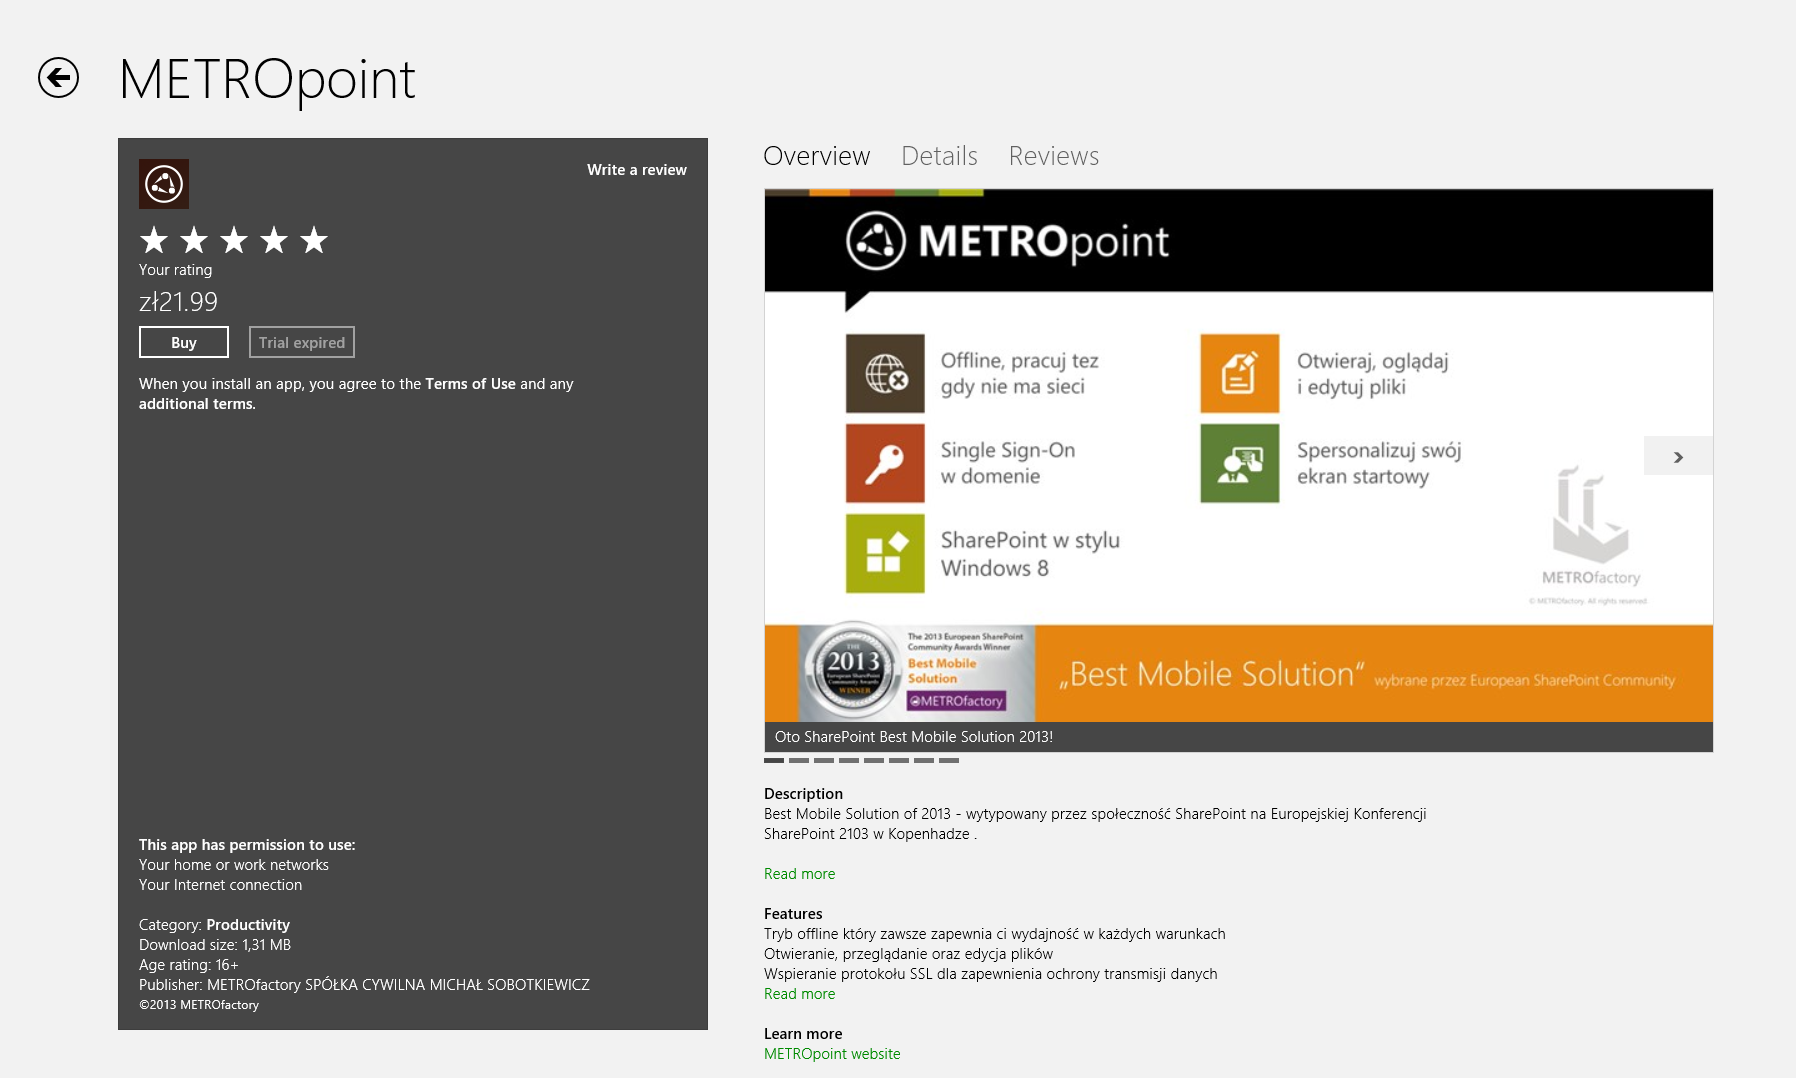
\includegraphics[width=\textwidth]{images/metropoint-shop.png}
\end{frame}

\begin{frame}
\frametitle{\textbf{METRO}point -- przykładowa aplikacja biznesowa}
 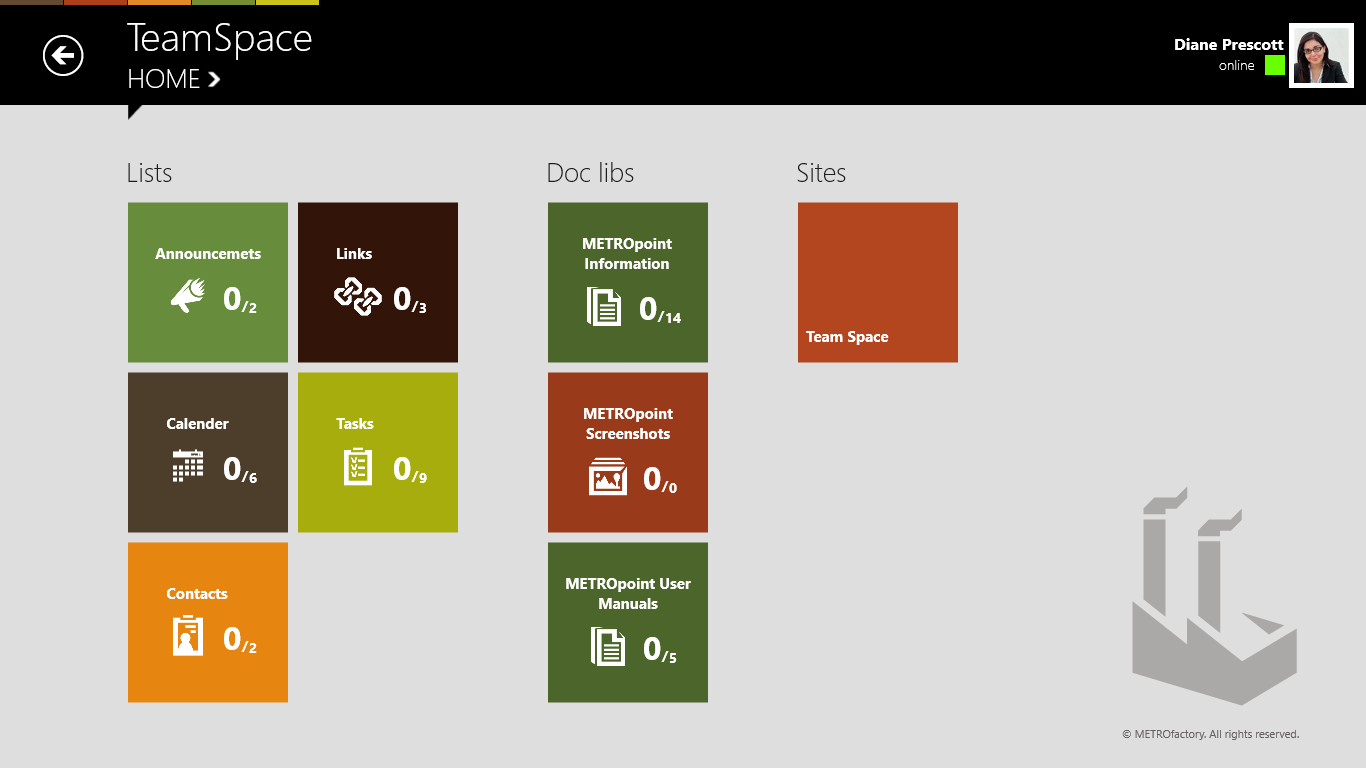
\includegraphics[width=\textwidth]{images/metropoint-screenshot.png}
\end{frame}

\begin{frame}
\frametitle{\textbf{METRO}point -- przykładowa aplikacja biznesowa}
 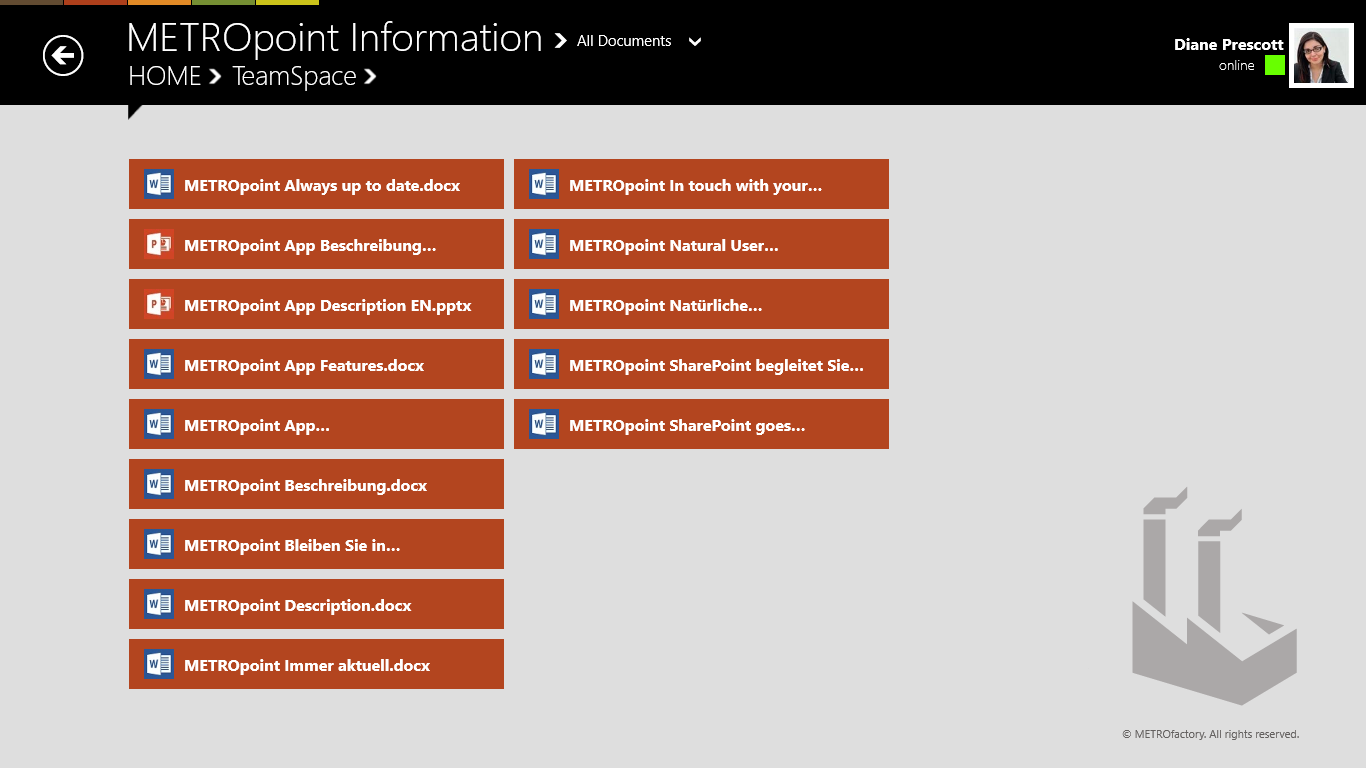
\includegraphics[width=\textwidth]{images/metropoint-document-list.png}
\end{frame}

\begin{frame}
\frametitle{\textbf{METRO}point -- przykładowa aplikacja biznesowa}
 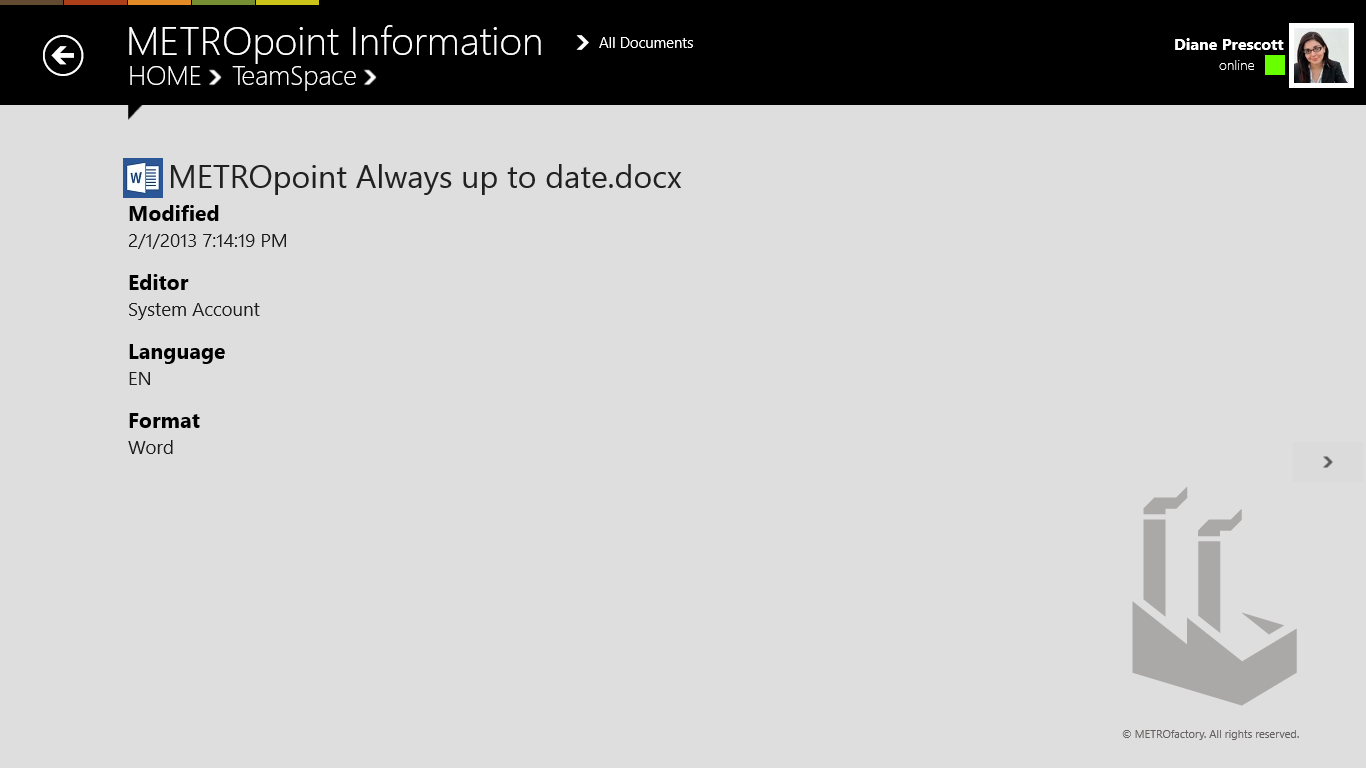
\includegraphics[width=\textwidth]{images/metropoint-document-details.png}
\end{frame}

\begin{frame}
\frametitle{\textbf{METRO}point -- możliwości}
\begin{itemize}[<+->]
\item Komunikacja z SharePoint 2010 oraz 2013
\item Personalizacja
\item Przystosowanie do urządzeń mobilnych 
\item Tryb Offline
\item Wykorzystanie wewnętrznych możliwości SharePoint
\end{itemize}
\end{frame}


\begin{frame}
\frametitle{\textbf{METRO}point -- branżowa nagroda}
 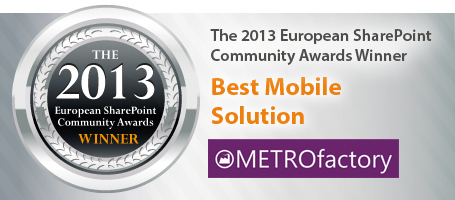
\includegraphics[width=\textwidth]{images/metrofactory-award.jpg}
\end{frame}

\begin{frame}
\frametitle{Zawartość części teoretycznej}
Opis użytych narzędzi podczas budowania aplikacji biznesowej razem z uzasadnieniem.
Między innymi:
\begin{itemize}[<+->]
\item Visual Studio 2012
\item Wzorzec architektoniczny MVVM
\item Język programowania \Csharp -- Nowości w wersji 5.0
\item Platforma Windows Runtime
\item Baza danych SQLite
\end{itemize}
\end{frame}

\begin{frame}
\frametitle{Zawartość części praktycznej}
Budowanie aplikacji, przy wykorzystaniu opisanych wcześniej narzędzi.

Poruszę takie tematy jak:
\begin{itemize}[<+->]
\item Analiza wymagań
\item Diagramy przypadków użycia
\item Schemat przepływu danych
\item Projekt modelu danych
\item Interfejs użytkownika
\end{itemize}
\end{frame}

\begin{frame}
\frametitle{Trudności w realizacji zadań pracy}

\begin{itemize}[<+->]
\item ,,Problemy wieku młodzieńczego'' Windows 8 oraz Windows Runtime.
\item Brak ,,dojrzałych'' bibliotek dla platformy Windows Runtime.
\item Ograniczenia sprzętowe.

\end{itemize}
\end{frame}


\begin{frame}
\frametitle{Bibliografia} 
\begin{itemize}
\item \href{http://msdn.microsoft.com/en-us/windows/apps/}{MSDN -- Windows Store apps}
\item \href{http://www.charlespetzold.com/blog/2013/01/Programming-Windows-6th-Edition-Final-Ebook-Now-Available.html}{Programming Windows 6th Edition -- Charles Petzold}
\end{itemize}
\end{frame}


\begin{frame}
\frametitle{Harmonogram} 
\begin{itemize}
\item czerwiec 2012 -- rozwój \textbf{METRO}point.
\item luty 2013 -- zbieranie potrzebnych źródeł danych, poszerzanie wiedzy na temat programowania w Windows 8.
\item lipiec 2013 -- rozpoczęcie pisania pracy inżynierskiej.
\end{itemize}
\end{frame}


\begin{frame}
\frametitle{Dziękuje za uwagę...}
Pytania?

\end{frame}

\end{document}
